\chapter{Uvod}
\thispagestyle{fancy}
\pagenumbering{arabic}
Motivacija za raziskavo je bilo ugotoviti do kakšne mere je mogoča razpoznavanje gibanja v živo na osnovi analize možganske aktivnosti z meritvami elektronecefalografije(EEG). Najprej smo podatke iz prosto dostopne zbirke podatkov s pomočjo knjižnice EEGLAB razdelili na nekaj različno dolgih epoh po dogodkih in jim zožili frekvenčne pasove. Iz vsake pridobljene zbirke podatkov smo pridobili matrike povezljivosti Grangerjevega indeksa vzročnosti in matrike povezljivosti kompleksnega Pearsonovega korelacijskega koeficienta. Na pridobljenih podatkih smo naučili nevronsko mrežo. Iz pridobljenih rezultatov smo se odločili za nadaljevanje razvoja na zbirki, ki je obetala najboljšo točnost. Da bi omogočili delovanje v realnem času smo sami implementirali nekaj že obstoječih funkcij iz knjižnice. Posneli smo podatke na napravi Cognionics Quick-20 in dodatno naučili nevronsko mrežo na naših podatkih za boljše razvrščanje.
\newpage
\section{Elektroencefalografija}
Elektroencefalografija(EEG) je metoda za merjenje možganske električne aktivnosti. Meri električne potenciale na površini temena ki jih deloma generira možganska aktivnost. V zadnjem stoletju so znanstveniki s pomočjo EEG pridobili vpogled v različne nevrološke bolezni. V zadnjem času pa se pojavlja interes v modeliranju EEG signalov in uporabo le teh za nadzor fizičnih naprav (ang. Brain-Computer Interfacing). EEG signali so običajno razdeljeni v frekvenčna območja, ki odražajo različne spektralne vrhove in jih povezujemo z različnimi možganskimi procesi. Ta območja so običajno določena kot delta (1-4 Hz), theta (4-8 Hz), alpha (8-13 Hz), beta (13-20 Hz), in gamma (>20 Hz). Slika \ref{slika:eeg}
 \cite{nunezElectroencephalographyEEGNeurophysics2016}
 \begin{figure}[h]
    \begin{center}
    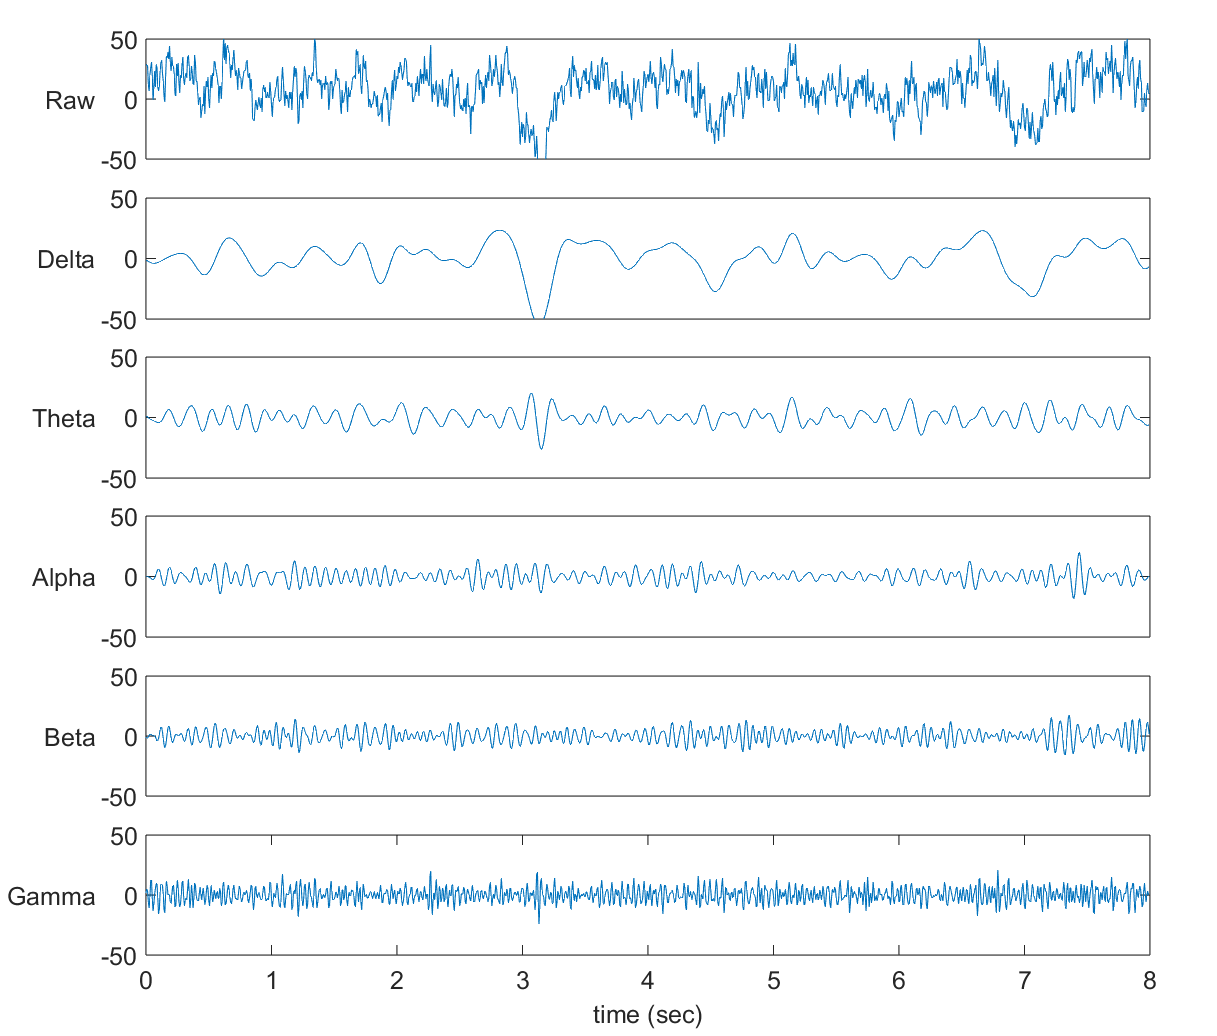
\includegraphics[width=1\linewidth]{slike/EEGSignals.png}
    \end{center}
    \caption[Frekvenčna območja EEG signala.]{Prvih 8 sekund EEG signala elektrode C3, osebe S001 serije R03. Od zgoraj navzdol po področjih: vsa skupaj, delta, theta, alpha, beta, gamma.}
    \label{slika:eeg}
    \end{figure}


\subsection{Mednarodni sitem 10-20 pozicioniranja elektrod}
Mednarodni sistem 10-20(slika \ref{slika:mednarodni_sistem_20}) standardizira mesta elektrod tako, da so te  nameščene v mrežo od naziona do iniona ter od desnega do levega sluhovoda v presledkih 10 in 20 odstotkov razdalje. Vsaka elektroda je označena s črko lokacijo: T-Temporal, F-Frontal, P-Parietal, C-Central in O-Occipital, ter s črko z za elektrode na sredini glave, lihimi številkami za levo polovico glave in sodimi za desno. \cite{klemTentwentyElectrodeSystem1999} Poleg mednarodnega sistema 10-20 za pozicioniranje elektrod obstajajo tudi drugi sistemi, kot je na primer mednarodni sistem 10-10 pozicioniranja elektrod. Podatki, snemani v živo, so bili pridobljeni po mednarodnem sistemu 10-20, medtem ko je bila podatkovna zbirka, uporabljena za učenje, snemana po prilagojenem mednarodnem sistemu 10-10 pozicioniranja elektrod.
\begin{figure}[h]
    \begin{center}
    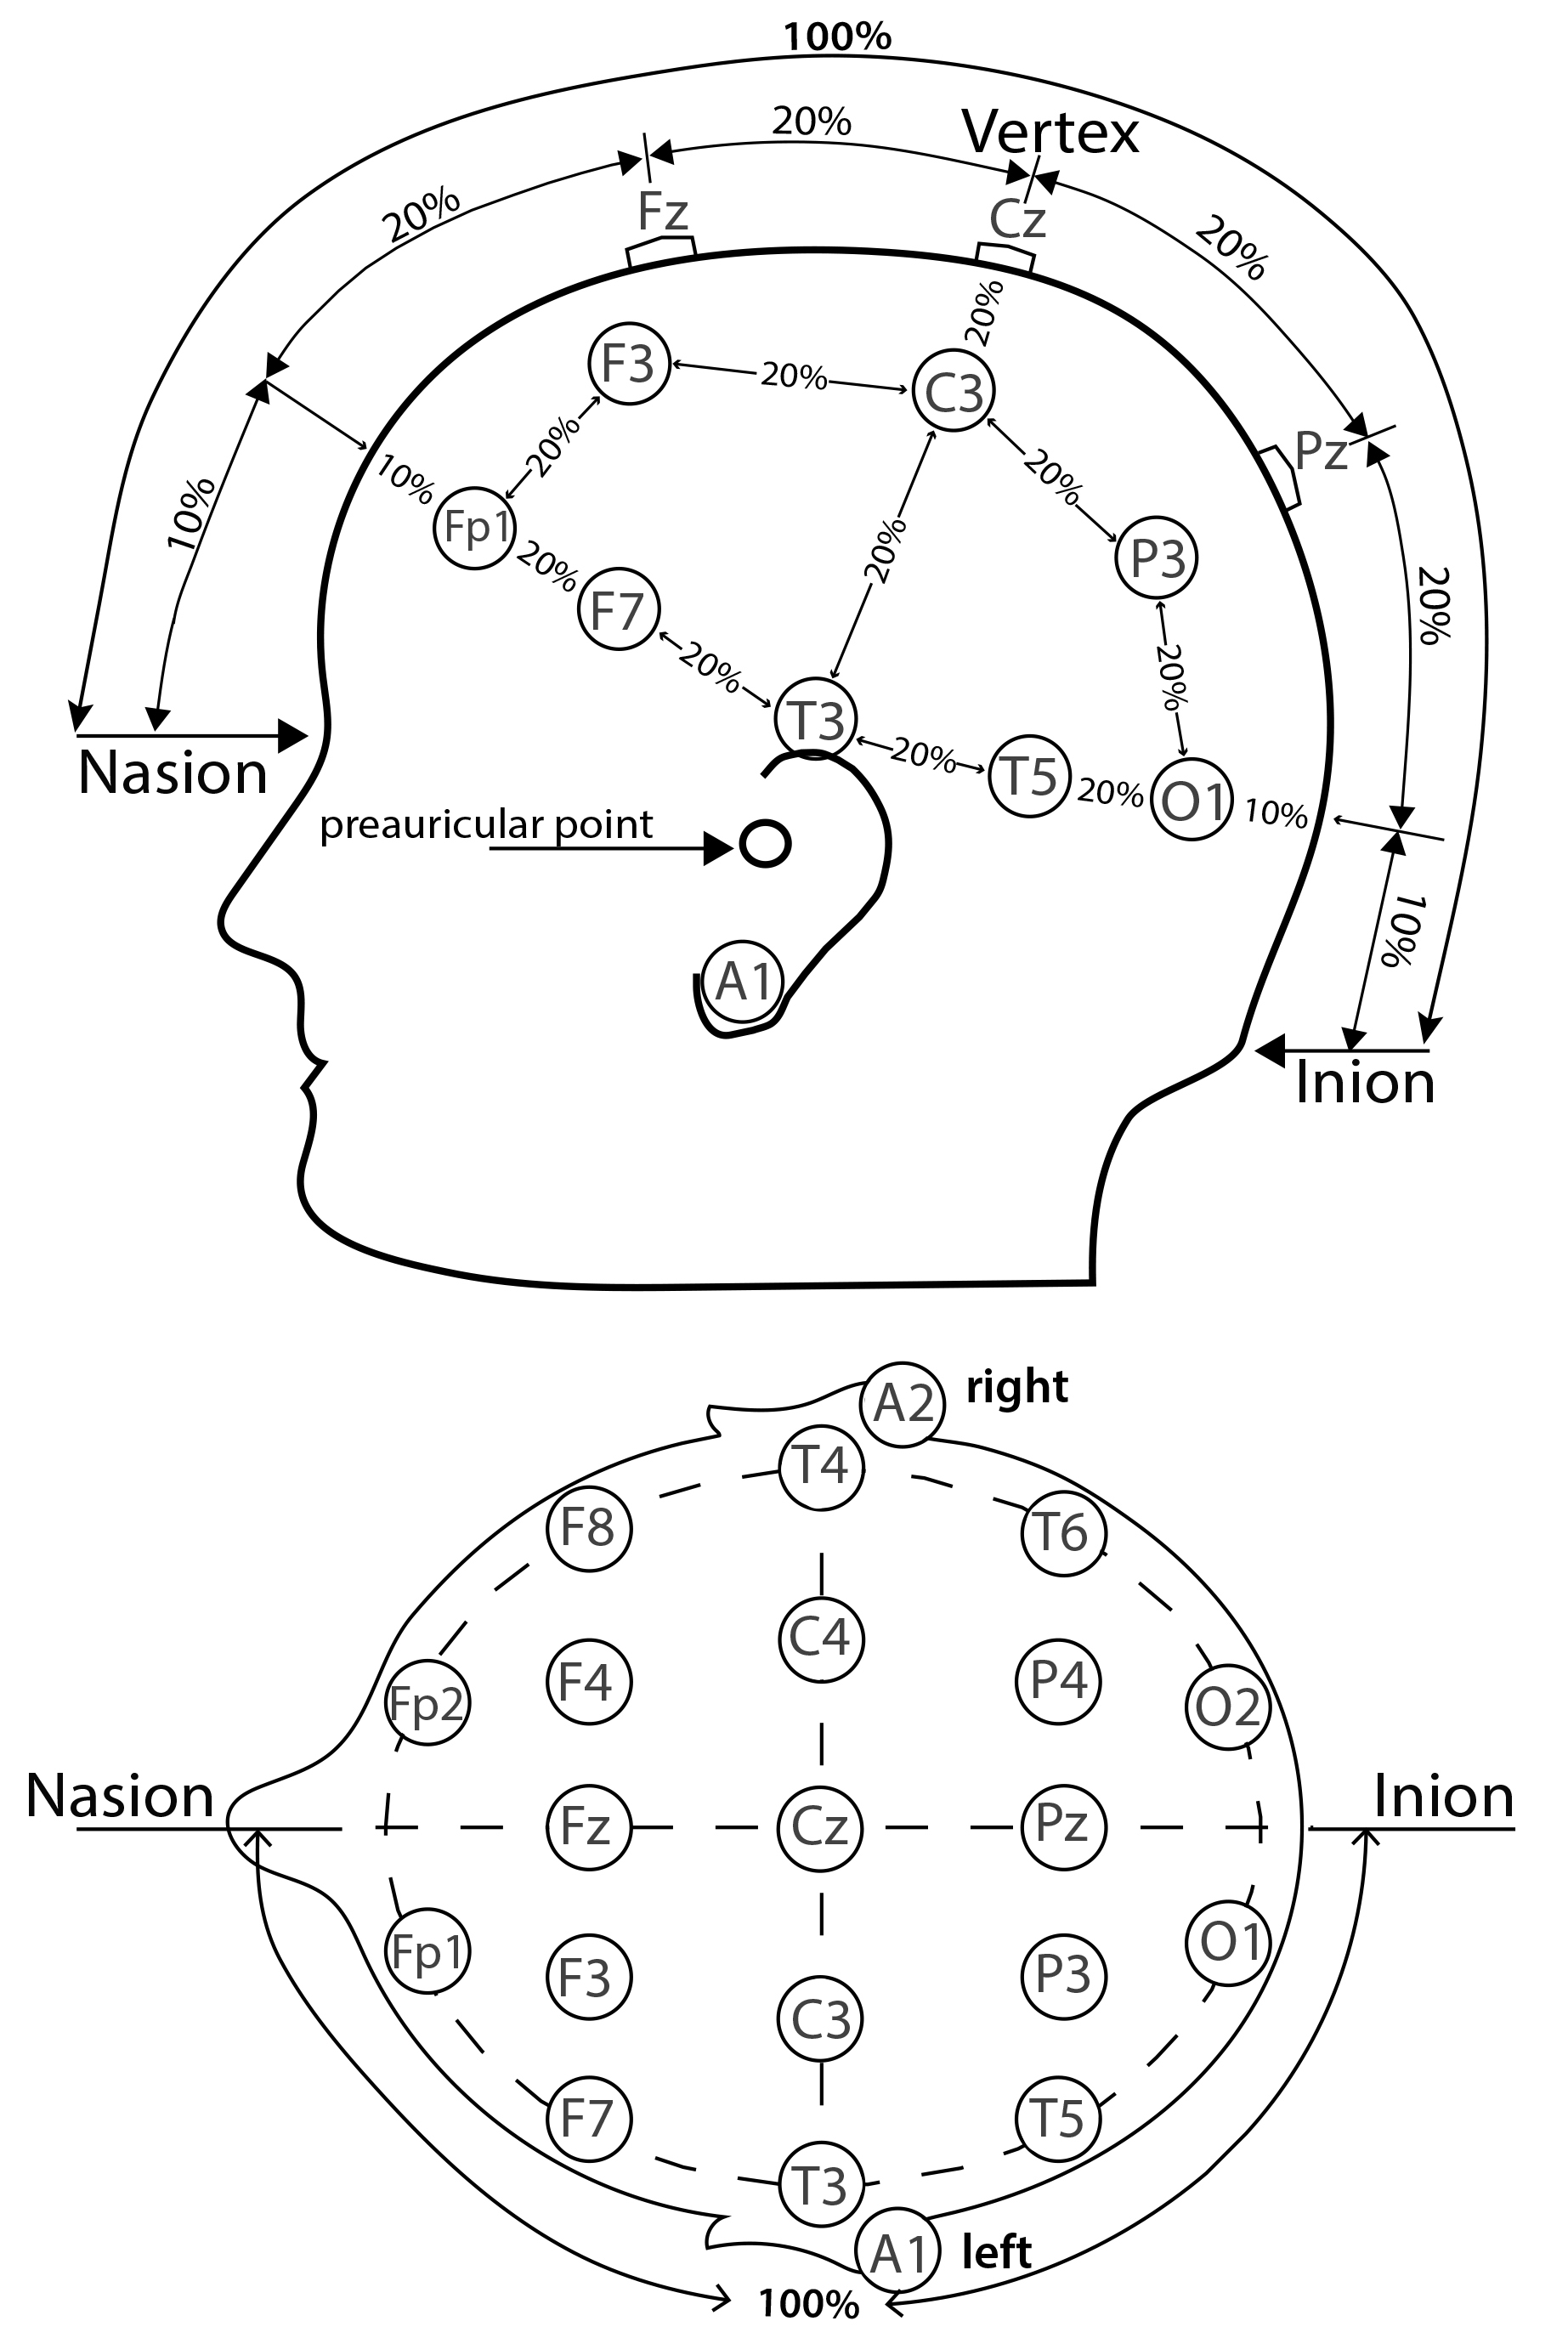
\includegraphics[width=0.5\linewidth]{slike/1020-diagram1.jpg}
    \end{center}
    \caption[Mednarodni sitem 10-20 pozicioniranja elektrod.]{Prikaz pozicije elektrod po mednarodnem sitemu 10-20. Nameščene v mrežo od naziona do iniona in od levega do desnega sluhovoda v presledkih 10 in 20 odstotkov. \cite{ElectrodeArrangementAccording}}
    \label{slika:mednarodni_sistem_20}
    \end{figure}

\begin{figure}
        \begin{center}
        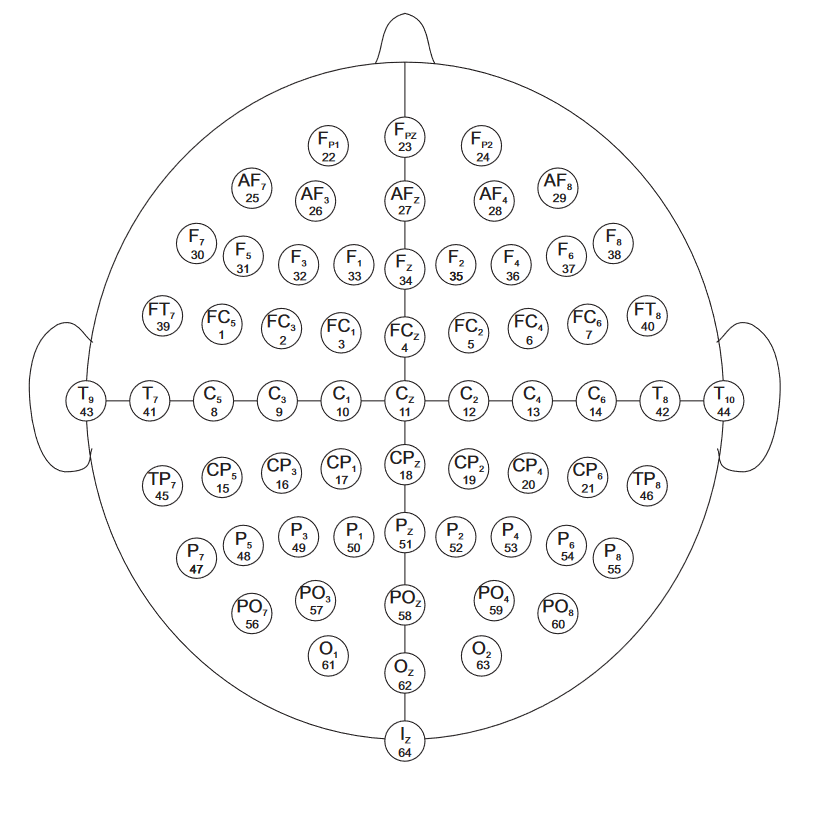
\includegraphics[width=1\linewidth]{slike/64electrodeSystem.png}
        \end{center}
        \caption[Mednarodni sitem 10-10 pozicioniranja elektrod.]{Prikaz pozicije elektrod po mednarodnem sitemu 10-10 pozicioniranja elektrod.  \cite{HttpsWwwPhysionet}}
        \label{slika:mednarodni_sistem_10}
        \end{figure}

\newpage

\subsection{Cognionics Quick-20}
Cognionics Quick-20(slika \ref{slika:quick_20}) je brezžična EEG naprava s suhimi elektrodami za raziskovalne namene. Ima 21 elektrod postavljenih po mednarodnem sitemu 10-20 za pozicioniranje elektrod. Naparava je suhega tipa kar pomeni, da pri uporabi elektrode ne potrebujejo gela. Suhi tipi naprav so v primerjavi z mokrimi enostavni in udobni za uporabo in omogočajo hitro nastavitev. Naprava je brezžična, z računalnikom jo povežemo preko USB vmesnika. \cite{DryEEGHeadset}

\begin{figure}[h!]
    \begin{center}
    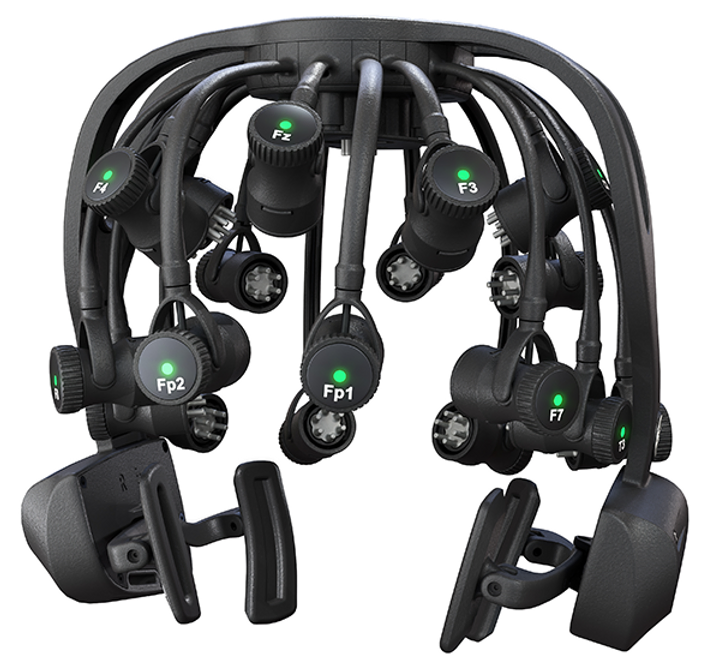
\includegraphics[width=0.5\linewidth]{slike/Cognionics Quick-20.png}
    \end{center}
    \caption{EEG naprava Cognionics Quick-20. \cite{CognionicsQUICK20User}}
    \label{slika:quick_20}
    \end{figure}
\section{Možganska povezljivost}
Možganska povezljivost se nanaša na vzorce nastale zaradi anatomskih povezav možganov, statistične odvisnosti ali interakcij med posameznimi deli možganov.  Enote med katerimi se meri povezljivost so lahko različne: posamezni nevroni, nevronske populacije, v našem primeru pa regije možganske skorje. Možganska aktivnost je omejena s povezljivostjo, le ta pa je zato ključnega pomena za razumevanje delovanja možganov. V grobem poznamo dve vrsti povezljivosti: strukturno in funkcijsko. Strukturna povezanost se nanaša na to kako so deli možganov med seboj fizično povezani. Funkcijska povezljivost pa se nanaša na to kako različni deli možganov med seboj komunicirajo oziroma sodelujejo.\cite{spornsBrainConnectivity2007} Funkcijsko povezljivost lahko nadaljnjo delimo na usmerjeno in neusmerjeno. V našem primeru je metoda Grangerjevega indeksa vzročnosti usmerjena saj je vpliv elektrode $A$ na elektrodo $B$ drugačen kot vpliv elektrode $B$ na elektrodo $A$. Metoda kompleksnega Pearsonovega korelacijskega koeficienta pa je neusmerjena saj nam njegova vrednost pove le o povezanosti para elektrod. Pri njej se ne ugotavlja smer vpliva.
V izrazu Grangerjev indeks vzročnosti je vzorčnost zavajajoč termin saj nam Grangerjev indeks vzročnosti nakazuje da ena stvar vpliva na drugo vendar sta lahko v določenih primerih obe meritvi odvisni od nečesa drugega. 
